%%%%%%%%%%%%%%%%%%%%%%%%%%%%%%%%%%%%%%%%%%%%%%%%%%%%%%%%%%%%%%%%%%%%%%%%%%%%%%%%
\chapter{Partitioning Algorithms}
\label{ch:part}
%%%%%%%%%%%%%%%%%%%%%%%%%%%%%%%%%%%%%%%%%%%%%%%%%%%%%%%%%%%%%%%%%%%%%%%%%%%%%%%%

We mentioned earlier that the microarray layout problem is usually approached in
two phases: placement and re-embedding. The placement, however, can be preceded
by a \emph{partitioning} phase that breaks the problem into smaller sub-problems
that are easier to manage. A partitioning algorithm divides the set of probes
$\mathcal{P}$ into smaller subsets, and assigns them to defined regions of the
chip. Each region can then be treated as an independent chip (and processed by a
placement algorithm) or be recursively partitioned. This is especially helpful
for placement algorithms with non-linear time or space complexities that are
otherwise unable to handle very large chips. Linear-time placement algorithms
may also benefit from a partitioning since probes with similar embeddings are
typically assigned to the same region --- Greedy and Row-Epitaxial
(Chapter~\ref{ch:placement}), for instance, are more likely to find good
candidates for filling the spots.

We describe four partitioning algorithms: 1-Dimensional Partitioning (1-DP),
2\hyph Dimensional Partitioning (2-DP), Centroid-based Quadrisection (CQ), and
Pivot Partitioning (PP). Like placement algorithms, they assume that an initial
embedding of the probes is given. Pivot Partitioning is the only algorithm that
modifies these embeddings.  As we shall see, 1-DP and 2-DP generate a few masks
with extremely few conflicts, but leave the remaining masks with many conflicts
that are difficult to handle, whereas CQ and PP offer a more uniform
optimization over all masks. Earlier results indicate that PP produces better
layouts than CQ on large chips \citep{Carvalho2006}.

Partitioning is clearly a compromise in solution quality since it restricts the
space of solutions and may lead to conflicts at partition borders, although it
can improve solution quality when the placement algorithm cannot handle large
regions well. Hence, it is not advisable to perform too many levels of
partitioning because smaller sub-regions mean less freedom for optimization
during placement. The right balance depends on the chip dimensions as well as on
the placement and partitioning algorithms.

%%%%%%%%%%%%%%%%%%%%%%%%%%%%%%%%%%%%%%%%%%%%%%%%%%%%%%%%%%%%%%%%%%%%%%%%%%%%%%%%
\section{1-Dimensional Partitioning}
\label{sec:part_1d}

The 1-Dimensional Partitioning algorithm \cite{Carvalho2007} divides the set of
probes based on the state of their embeddings at a particular synthesis step. It
starts by creating two subsets of $\mathcal{P}$:
%%
\[
\mathcal{P}_0 = \{ p_k \in \mathcal{P} | \eps_{k,1} = 0 \},
\qquad
\mathcal{P}_1 = \{ p_k \in \mathcal{P} | \eps_{k,1} = 1 \}.
\]

In other words, $\mathcal{P}_0$ contains all probes whose embeddings are
unproductive during the first synthesis step, whereas $\mathcal{P}_1$ contains
probes with productive embeddings. The chip is then divided into two horizontal
(or vertical) bands, proportionally to the number of probes in $\mathcal{P}_0$
and $\mathcal{P}_1$, so each band accommodates one subset of $\mathcal{P}$.

This procedure is recursively applied to each band, using the the next synthesis
steps to further divide each subset of probes. For instance, the following
subsets of $\mathcal{P}_0$ and $\mathcal{P}_1$ are created during step $t=2$:
%%
\[
\mathcal{P}_{00} = \{ p_k \in \mathcal{P}_0 | \eps_{k,2} = 0 \},
\qquad
\mathcal{P}_{01} = \{ p_k \in \mathcal{P}_0 | \eps_{k,2} = 1 \},
\]
\[
\mathcal{P}_{10} = \{ p_k \in \mathcal{P}_1 | \eps_{k,2} = 0 \},
\qquad
\mathcal{P}_{11} = \{ p_k \in \mathcal{P}_1 | \eps_{k,2} = 1 \}.
\]

\begin{figure}\centering
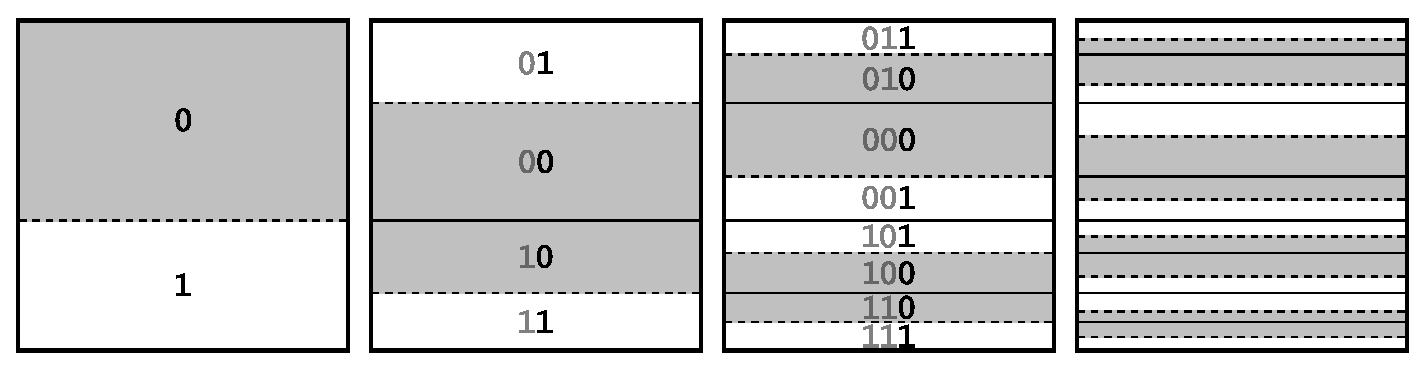
\includegraphics[width=\textwidth]{1dpart.eps}
\caption{\label{fig:1dpart}%
  First four levels of 1-Dimensional Partitioning. Dashed lines show the
  divisions performed in each step; solid lines indicate regions delimited in
  previous steps (there are no border conflicts between spots separated by
  solid lines). Masked (shaded) regions are labeled ``0'',
  unmasked (white) regions are labeled ``1''. This labeling forms
  a binary Gray code (shown in the first three steps only).}
\end{figure}

The next assignments of subsets to the upper or lower band of their regions are
made in such a way that regions with the same ``state'' --- productive
(unmasked) or unproductive (masked) --- are joined as far as possible, resulting
in masks that consist of alternating layers of masked and unmasked spots. This
process is illustrated in Figure~\ref{fig:1dpart}, where at each step~$t$, a
band is labeled ``0'' when its embeddings are unproductive, and ``1'' when its
embeddings are productive. The resulting binary numbers from top to bottom form
a binary Gray code, that is, a permutation of the binary numbers between 0 and
$2^n - 1$ such that neighboring elements differ in exactly one bit, as do the
first and last elements \citep{Kreher1999}.

The Gray code highlights an interesting property of 1-DP. After $d$~levels of
partitionings (based on steps $1$ to $d$), the embeddings of any two immediate
neighbors differ among the first $d$~steps in at most one step.  As a result,
masks $M_1$ to $M_d$ exhibit a layered structure that effectively reduces
border conflicts. The Gray code is disrupted as soon as a region cannot be
divided (because all probes of that region are masked at a particular step,
for instance). This will certainly happen as several binary numbers are unlikely
to be substrings of embeddings (for example, numbers containing long runs of
zeros).

Moreover, 1-DP can optimize only a limited number of masks because the
sub-regions soon become too narrow to be further divided. The maximum
\emph{partitioning depth} $d_{max}$ is primarily limited by the number of rows
(or columns) on the chip. In practice, since regions are likely to be unevenly
divided, $d_{max}$ varies between regions. The algorithm can also be configured
to stop partitioning a region once its height drops below a given threshold
$H_{max}$ (i.e., the maximum height of any final region will not exceed
$H_{max}$).

1-DP is easier to implement if the partitionings always produce rectangular
regions (i.e., splitting a row between two regions is not allowed). In order to
force an exact division of a region, however, it might be necessary to move a
few probes from one subset of probes to the other one.

For example, imagine that a chip with $|\mathcal{P}| = 900$ probes, $n_r = 30$
rows and $n_c = 30$ columns is to be partitioned based on the state of the
embeddings at the first synthesis step, resulting in sub-sets $\mathcal{P}_0$
and $\mathcal{P}_1$ with, say, 638 and 262 probes, respectively. The chip must
thus be divided into two sub-regions, the upper one containing
$[30 \cdot 638/900]=21$ rows and the lower one with $[30 \cdot 262/900]=9$ rows
(where $[x]$ denotes the nearest integer of $x$). The problem is that the upper
region then contains $21 \cdot 30 = 630$ spots but it has to accommodate 638
probes, whereas the lower region contains $9 \cdot 30 = 270$ spots but only 262
probes. The solution is to (arbitrarily) move 8 probes from $\mathcal{P}_0$ to
$\mathcal{P}_1$, which results in some imperfections in the layers of the
corresponding mask (a few masked spots in a region of unmasked spots and
vice-versa).

%%%%%%%%%%%%%%%%%%%%%%%%%%%%%%%%%%%%%%%%%%%%%%%%%%%%%%%%%%%%%%%%%%%%%%%%%%%%%%%%
\section{2-Dimensional Partitioning}
\label{sec:part_2d}

\begin{figure}[t]\centering
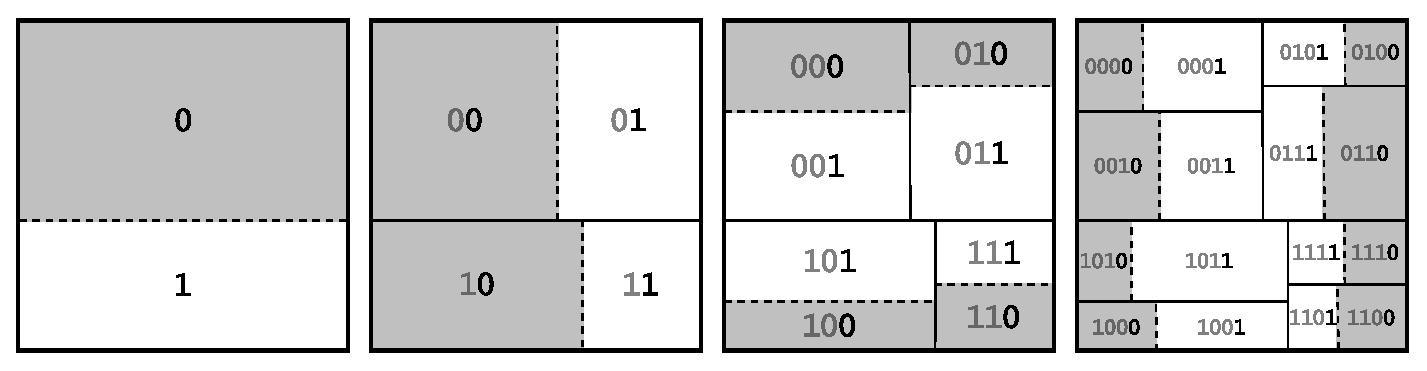
\includegraphics[width=\textwidth]{2dpart.eps}
\caption{\label{fig:2dpart}%
  First four levels of 2-Dimensional Partitioning. Dashed lines show the
  divisions performed in each step; solid lines indicate regions delimited in
  previous steps. Masked regions are labeled with ``0'', unmasked regions with
  ``1''; this labeling forms an approximation to a two-dimensional binary Gray
  code.}%
\end{figure}

The 2-Dimensional Partitioning algorithm \cite{Carvalho2007} extends the idea of
1-DP to two dimensions, with the potential of optimizing twice as many masks.
The algorithm is similar: $\mathcal{P}$ is divided into subsets based on the
state of the embeddings at a particular synthesis step. The differences are that
2-DP alternates horizontal and vertical divisions of regions, and that the
assignments of probes to regions obey a two-dimensional binary Gray code (Figure
\ref{fig:2dpart}). In a 2-D Gray code, the binary numbers are arranged in a
matrix in such a way that two neighboring numbers differ in at most one bit. As
a result, regions whose embeddings are at the same state (productive or
unproductive) are joined as far as possible.

If regions were always equally divided, 2-DP would have the same property as 1-
DP: After $d$~levels of partitionings, the
embeddings of any two immediate neighbors would differ among the first $d$ steps
in at most one step. However, this is not always the case since 2-DP is likely
to create regions with different dimensions, forcing some regions to share a
border with more than its four natural neighbors. For instance, in
Figure~\ref{fig:2dpart} region ``0010'' borders with ``0000'', ``1010'', and
``0011'', but also with ``0001'' and ``1011''.

Like 1-DP, the maximum partitioning depth, $d_{max}$, is limited by the number
of rows and columns on the chip, and it varies since regions are likely to be
unevenly divided. 2-DP can also be configured to stop partitioning a region as
soon as its dimensions (height and width) drop bellow a given threshold
$L_{max}$ (the largest final region will contain at most ${L_{max}}^2$ spots).

Figure \ref{fig:2dpart_bl} shows the normalized border length per masking step
of layouts produced by 2-DP for a random $1\,000\times 1\,000$ chip. With maximum
partitioning depth ($L_{max}=1$), 2-DP produced a layout with the best masks for
the first 22 synthesis steps. However, because the chip is partitioned until all
regions contain a single probe, the placement algorithm has no freedom for
reducing border conflicts in the remaining masks. As a result, after step 32,
the levels of border conflicts are as high as in the random layout.

With $L_{max}=10$, there is more room for optimization during placement since
the final regions can be as large as $10\times 10$. In this case, we used the
Greedy placement algorithm (Section~\ref{sec:placement_greedy}) with $Q=100$ so
that all probes of a region were considered for filling its spots. This resulted
in a reduction of about $13.4\%$ in normalized border length compared to the
layout produced with $L_{max}=1$ (from $21.5588$ to $18.6670$, data not shown),
although we observed an increase of border conflicts in the first 24 masks.
Increasing $L_{max}$ even further to 50 and using Greedy with $Q=2\,500$
resulted in a reduction of $8.1\%$ in normalized border length compared to
$L_{max}=10$ (from $18.6670$ to $17.1629$) but, again, this came at the expense
of an increase of border conflicts in the first 20 masks.

\begin{figure}[t]\centering
\includegraphics{part/2dpart/bl}
\caption{\label{fig:2dpart_bl}
  Normalized border length per masking step of several layouts for a
  $1\,000\times 1\,000$ chip with random probes left-most embedded in the
  standard Affymetrix depostion sequence: random layout ({\tiny $\boxdot$}); 2-D
  Partitioning with $L_{max}=1$ ({\scriptsize $\times$}); 2-D Partitioning with
  $L_{max}=10$ and Greedy placement with $Q=100$ ({\tiny $\odot$}); 2-D
  Partitioning with $L_{max}=50$ and Greedy placement with $Q=2\,500$
  ({\tiny $+$}).}
\end{figure}

Figure~\ref{fig:1dp_versus_2dp} compares the results obtained by 1-DP and 2-DP
on the same $1\,000\times 1\,000$ chip of Figure \ref{fig:2dpart_bl}. We first
compare both algorithms with their maximum partitioning depths ($H_{max}=1$ for
1-DP and $L_{max}=1$ for 2-DP). With $L_{max}=1$, 2-DP produces $1\times 1$
regions and leaves no room for optimization during placement. In constrast, 1-DP
with $H_{max}=1$ produces regions with a single row but, in this case, with
$1\,000$ columns (and $1\,000$ probes), leaving a considerable degree of
freedom for the placement algorithm. To be fair, we thus compare 1-DP and
2-DP using a placement algorithm that places probes randomly inside each final
region, so that the results are only due to the partitionings (and not to the
placement algorithm). In our results, with maximum partitioning depths, 1-DP and
2-DP produced layouts with similar levels of border conflicts in masks
$M_{33}$ to $M_{74}$, although the layout produced by 2-DP was slightly better
in masks $M_{58}$ to $M_{69}$. However, while 1-DP was able to produce masks
with relatively few conflicts in the first 17 steps, 2-DP achieved even greater
reductions of border conflicts in the first 32 steps. The normalized border
length of these layouts are $25.8543$ (with 1-DP) and $21.5588$ (with 2-DP).

In Figure~\ref{fig:1dp_versus_2dp} we also compare 1-DP with $H_{max}=1$ and
2-DP with $L_{max}=50$ using Greedy for the placement. With $L_{max}=50$, 2-DP
produces regions containing at most $2\,500$ probes. For this particular chip,
2-DP produced $1\,005$ regions, containing $995.02$ probes on average (the
largest region contained $2\,209$ and the smallest $210$ probes), so Greedy had
about the same degree of freedom provided by 1-DP with $H_{max}=1$. We used a
sufficiently large number $Q$ of candidates per spot so that all probes of a
region were considered for filling its spots. With these settings, the layouts
produced by 1-DP and 2-DP have similar levels of border conflicts in masks
$M_{20}$ to $M_{74}$. In the first 18 synthesis steps, however, 2-DP produced
better masks, especially after step 5. The normalized border length of these
layouts are $18.0078$ (1-DP) and $17.1629$ (2-DP).

\begin{figure}[t]\centering
\includegraphics{part/1d_versus_2d/bl}
\caption{\label{fig:1dp_versus_2dp}
  Normalized border length per masking step of layouts produced by 1-D and 2-D
  Partitioning for a $1\,000\times 1\,000$ chip with random probes left-most
  embedded in the standard Affymetrix depostion sequence: 1-DP with $H_{max}=1$
  and random placement ({\scriptsize $\times$}); 2-DP with $L_{max}=1$
  ({\tiny $\boxdot$}); 1-DP with $H_{max}=1$ and Greedy placement with
  $Q=1\,000$ ({\tiny $+$}); 2-DP with $L_{max}=50$ and Greedy placement with
  $Q=2\,500$ ({\tiny $\odot$}).}
\end{figure}

A representation of selected photolithographic masks generated by 2-DP for a
$300\times 300$ chip are shown in Figure \ref{fig:2dpart_masks}. The resulting
rectangular regions can be clearly seen up to mask $M_{18}$. In the first
eight masks it is possible to see some ``imperfections'' (unmasked spots on
masked regions or vice-versa) that result from arbitrarily moving probes between
regions in order to force exact divisions. On a chip of this size, 2-DP can
usually reduce conflicts up to the $25^{\mathrm{th}}$ synthesis step, although
this is not noticeable in $M_{25}$ of Figure \ref{fig:2dpart_masks}.

\begin{figure}[p]\centering
%%
\begin{picture}(435,567)\footnotesize{
\put( -2,439){\makebox(145,128){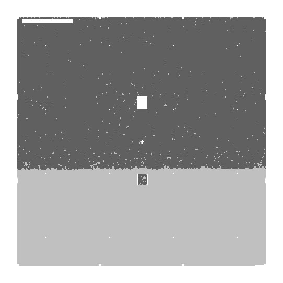
\includegraphics{part/2dmasks/mask01}}}
\put(147,439){\makebox(145,128){
\includegraphics{part/2dmasks/mask02}}}
\put(292,439){\makebox(145,128){
\includegraphics{part/2dmasks/mask03}}}
\put( -2,429){\makebox(145, 10){$M_1$}}
\put(147,429){\makebox(145, 10){$M_2$}}
\put(292,429){\makebox(145, 10){$M_3$}}
\put( -2,296){\makebox(145,128){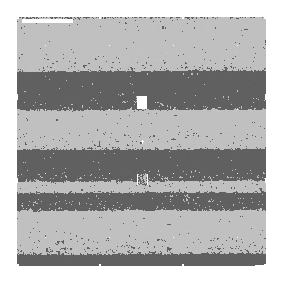
\includegraphics{part/2dmasks/mask04}}}
\put(147,296){\makebox(145,128){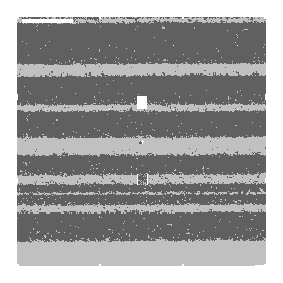
\includegraphics{part/2dmasks/mask05}}}
\put(292,296){\makebox(145,128){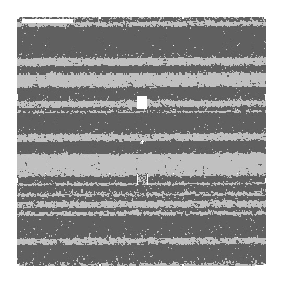
\includegraphics{part/2dmasks/mask06}}}
\put( -2,286){\makebox(145, 10){$M_4$}}
\put(147,286){\makebox(145, 10){$M_5$}}
\put(292,286){\makebox(145, 10){$M_6$}}
\put( -2,153){\makebox(145,128){
\includegraphics{part/2dmasks/mask07}}}
\put(147,153){\makebox(145,128){
\includegraphics{part/2dmasks/mask08}}}
\put(292,153){\makebox(145,128){
\includegraphics{part/2dmasks/mask13}}}
\put( -2,143){\makebox(145, 10){$M_7$}}
\put(147,143){\makebox(145, 10){$M_8$}}
\put(292,143){\makebox(145, 10){$M_{13}$}}
\put( -2, 10){\makebox(145,128){
\includegraphics{part/2dmasks/mask18}}}
\put(147, 10){\makebox(145,128){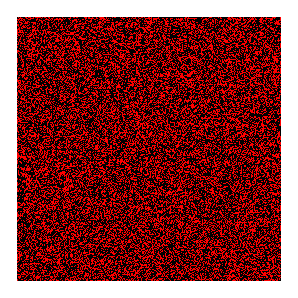
\includegraphics{part/2dmasks/mask25}}}
\put(292, 10){\makebox(145,128){
\includegraphics{part/2dmasks/mask68}}}
\put( -2,  0){\makebox(145, 10){$M_{18}$}}
\put(147,  0){\makebox(145, 10){$M_{25}$}}
\put(292,  0){\makebox(145, 10){$M_{68}$}}
}\end{picture}
%%
\caption{\label{fig:2dpart_masks}%
  Selected masks generated by 2-Dimensional Partitioning with $L_{max}=1$ for a
  random $300\times 300$ chip with 25-mer probes left-most embedded into the
  standard Affymetrix deposition sequence. Unmasked (masked) spots are
  represented by light (dark) dots.}
\end{figure}

So far we have described both 1-DP and 2-DP using the state of the first $d$
synthesis steps to divide the set of probes. The result of this approach is
that, while the first masks are optimized, the remaining masks are left with
high levels of border conflicts; we call this a \emph{left-most mask
optimization}.

However, a defect in the middle of the probe is more harmful than in its
extremities, so it is more important to optimize the central masks that are more
likely to add the middle bases. Fortunately, it is possible to reduce conflicts
in the central masks using 1-DP and 2-DP by partitioning the probe set based on
the following sequence of synthesis steps, assuming that $T$ is even and $d$ is
odd:
$T/2, (T/2)\pm 1, (T/2)\pm 2, \dots, (T/2)\pm\lfloor d/2\rfloor$; we call this a
\emph{centered mask optimization}.

\begin{figure}[t]\centering
\includegraphics{part/left_versus_central/bl}
\caption{\label{fig:2d_left_center}
  Normalized border length per masking step (on the left y-axis) of two layouts
  produced by 2-Dimensional Partitioning with $L_{max}=50$ and Greedy placement
  with border length minimization and $Q=2.5$K for a $1\,000 \times 1\,000$ chip
  with random probe sequences: left-most mask optimization with left-most
  embeddings ({\tiny $\boxdot$}); centered mask optimization with centered
  embeddings ({\scriptsize $\times$}). The number of middle bases synthesized at
  each step (with centered embeddings) is shown in boxes (right y-axis).}
\end{figure}

For left-most optimization, it makes sense to embed the probes in a left-most
fashion in order to reduce conflicts in the last masks (which are not optimized
by the partitioning). The left-most embeddings reduce the number of unmasked
spots in the last steps, resulting in masks that largely consist of masked
spots and consequently low levels of border conflicts. In contrast, centered
mask optimization produces better results with \emph{centered} embeddings. A
centered embedding is constructed by shifting a left-most embedding to the right
until the number of masked steps to the left of the first productive step is
approximately equal to the number of masked steps to the right of the last
productive step.

\ignore{An aligned
embedding is constructed by shifting a left-most embedding in such a
way that the middle base is added during the middle cycle (or as
close as possible to it).
}%% aligned embeddings are giving worse results than centered embeddings

Figure~\ref{fig:2d_left_center} shows the results of using 2-D Partitioning with
$L_{max}=50$ on a $1\,000\times 1\,000$ chip with left-most and centered mask
optimization. With left-most mask optimization, we obtain a normalized border
length of $17.1629$ (up to approximately $0.32$ per step). With centered mask
optimization, the normalized border length improves by $1.03\%$ to $16.9855$
(not shown in the figure). The average conflict index, however, is reduced by as
much as $34.89\%$ (from $577.3353$ to $375.9232$) because of the higher weight
of the middle bases in the conflict index measure.

\begin{table}[t!]\centering
\caption{\label{tab:2dp_greedy}
  Average conflict index (ACI) of layouts produced by Greedy placement and 2-D
  Partitioning on random $800\times 800$ chips with left-most and centered
  embeddings. 2-DP was configured for centered mask optimization and used Greedy
  for the placement. In all cases, Greedy was configured for conflict index
  minimization and used $0$-threading. Results are averages over a set of five
  arrays and running times are reported in minutes.}
\footnotesize{
\begin{tabular}{clrr}
Embeddings & Algorithm & ACI & Time \\
\hline
Left-most  & Greedy with $Q=20$K & 392.1786 & 186.4 \\
Left-most  & Greedy with $Q=40$K & 378.3110 & 357.0 \\
Left-most  & Greedy with $Q=80$K & 366.8446 & 680.9 \\
\hline
Centered   & Greedy with $Q=20$K & 387.5974 & 205.1 \\
\hline
Centered   & 2-DP with $L_{max}=10$ and Greedy with $Q=100$    &      345.9908  & 0.6 \\
Centered   & 2-DP with $L_{max}=20$ and Greedy with $Q=400$    &      342.2031  & 1.3 \\
Centered   & 2-DP with $L_{max}=30$ and Greedy with $Q=900$    & {\bf 341.2786} & 2.3 \\
Centered   & 2-DP with $L_{max}=40$ and Greedy with $Q=1\,200$ &      341.6185  & 4.0 \\
Centered   & 2-DP with $L_{max}=50$ and Greedy with $Q=2\,000$ &      341.7515  & 6.1 \\
Centered   & 2-DP with $L_{max}=60$ and Greedy with $Q=3\,600$ &      341.8634  & 8.4 \\
\hline
\end{tabular}}
\end{table}

%% data removed from table {tab:2dp_greedy}
%% Centered   & 2-DP with $L_{max}=25$ and Greedy with $Q=625$    &      341.4105  & 1.8 \\
%% Centered   & 2-DP with $L_{max}=35$ and Greedy with $Q=1\,225$ & {\bf 341.2372} & 2.7 \\

When carefully used, 1-DP and 2-DP can improve placement by producing a few
masks with very low levels of border conflicts, and breaking the problem into
smaller sub-problems that are easier to handle. Table \ref{tab:2dp_greedy} shows
results on $800\times 800$ arrays using 2-DP with centered mask optimization and
Greedy with conflict index minimization for the placement, in comparison to
using Greedy alone (results with Greedy as shown on Table \ref{tab:greedy} and
Figure \ref{fig:greedy_tradeoff}). Results of Greedy with centered embeddings
are also shown. In our results, the layouts produced by 2-DP are even better
than the ones produced by Greedy with $Q=80$K. This is a consequence of the
importance of the middle bases in the conflict index measure. Moreover, while
Greedy required about $680.9$ minutes with $Q=80$K, the combination of 2-DP and
Greedy required at most $8.4$ minutes because the partitioning restricts the
number of candidates Greedy can look at for each spot.

Increasing $L_{max}$ provides more room for optimization during placement but
worsens the central masks, while reducing $L_{max}$ improves the central masks
at the expense of an increase of conflicts in the remaining masks (in this case,
reducing $L_{max}$ also improves running time as Greedy has fewer candidates
available for each spot). The best trade-off depends on several aspects of the
problem such as chip dimension, probe embeddings, type of optimization (border
length or conflict index), and placement algorithm. For this case, the best
results were achieved with $L_{max}=30$.

%%%%%%%%%%%%%%%%%%%%%%%%%%%%%%%%%%%%%%%%%%%%%%%%%%%%%%%%%%%%%%%%%%%%%%%%%%%%%%%%
\section{Centroid-based Quadrisection}
\label{sec:part_cq}

\begin{figure}\centering
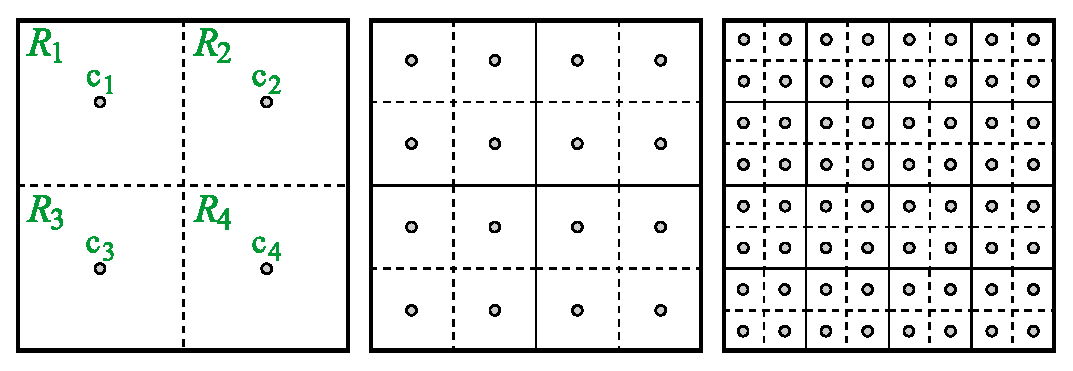
\includegraphics[width=\textwidth]{quadrisect.eps}
\caption{\label{fig:quadrisect}%
  First three levels of Centroid-based Quadrisection. Dashed lines show the
  divisions performed in each step; solid lines indicate regions delimited in
  previous steps. The centroids of each partition $R_{c_1}$ to $R_{c_4}$ are
  represented by small circles (labeled with $p_{c_1}$ to $p_{c_4}$ in the
  first step).}
\end{figure}

Centroid-based Quadrisection \citep{Kahng2003a}, CQ for short, employs a
different criterion for dividing the probe set and a different approach for
partitioning. At each iteration, a region $R$ is quadrisectioned into $R_{c_1}$,
$R_{c_2}$, $R_{c_3}$, and $R_{c_4}$. Each sub-region $R_{c_i}$ is associated
with a selected probe $p_{c_i}\in \mathcal{P}$, called \emph{centroid}, that is
used to guide the assignment of the remaining probes to the sub-regions.

A centroid is a representative of its region: It should symbolize the ``average
embedding'' in that region. The remaining probes
$p_k \in \CalP \setminus \{p_{c_1},p_{c_2},p_{c_3},p_{c_4}\}$ are compared to
each centroid and assigned to the sub-region $R_{c_i}$ whose centroid minimize
the Hamming distance $H(k,c_i)$ (as defined in Section
\ref{sec:mlp_border_length}).

The authors argue that, in order to improve the ``clustering'' of similar
probes, the four centroids should be as different from each other as possible.
The following heuristic is proposed: First, a probe index $c_1$ is randomly
selected from $\{1,\dots,|\mathcal{P}|\}$.  Then, a probe index $c_2\neq c_1$
maximizing $H(c_2,c_1)$ is selected.  Similarly, $c_3$ maximizing
$H(c_3,c_1) + H(c_3,c_2)$ and $c_4$ maximizing
$H(c_4,c_1) + H(c_4,c_2) + H(c_4,c_3)$ are selected.  The assignment of
centroids to the quadrisections of the chip is arbitrary.

Since the partitioning must always produce four regions of the same size,
sometimes it is necessary to make non-optimal assignment of probes to regions.
In order to recover from a possibly bad choice of centroids, a ``multi-start
heuristic'' is used, running the centroid selection procedure several times with
different ``seeds'' for $c_1$ and keeping the centroids that lead to the best
partitioning. For measuring partitioning quality, the algorithm uses the sum of
Hamming distances between the embeddings of the probes and the embedding of the
centroid (the partitioning that results in the least sum is selected).

The maximum partitioning depth $d_{max}$ of CQ is $\log_2 n_r$, assuming that
$n_r$ is a power of 2 and that $n_c=n_r$ ($n_r$ and $n_c$ are the number of rows
and columns on the chip, respectively). In practice, the partitioning continues
until a pre-defined depth $D$ has been reached.

Although CQ was developed for border length minimization (BLM), it can be
adapted for conflict index minimization (CIM) by using the \emph{conflict index
distance} $C(k,k')$ (as defined in Section \ref{sec:mlp_conflict_index}) instead
of the Hamming distance $H(k,k')$ for selecting the centroids as well as for
deciding which partition a probe should be assigned to.

As mentioned in Section \ref{sec:placement_greedy}, placement algorithms such as
Row-Epitaxial and Greedy have the drawback of treating the last $Q - 1$ filled
spots unfairly since fewer than $Q$ probe candidates are available to fill them.
This issue is aggravated by a partitioning because in each final partition
$Q - 1$ spots have fewer than $Q$ probe candidates. In order to attenuate this
problem, a \emph{borrowing heuristic} was implemented in CQ to allow the
placement algorithm (Row-Epitaxial, in the original implementation) to look at
$Q$ probes ``in the current and the next region''. Although the authors did not
specify the exact meaning of ``next region'', it can be, for instance, the next
region to be processed by the placement algorithm. Borrowing probes from a
region $R_{c_i}$ to fill spots of $R_{c_j}$ obviously requires using the
unplaced probes of $R_{c_j}$ to fill spots of $R_{c_i}$.

%%%%%%%%%%%%%%%%%%%%%%%%%%%%%%%%%%%%%%%%%%%%%%%%%%%%%%%%%%%%%%%%%%%%%%%%%%%%%%%%
\section{Pivot Partitioning}
\label{sec:part_pp}

Pivot Partitioning \citep{Carvalho2006}, PP for short, is to a certain extent
similar to CQ: Sub-regions are recursively associated with special probes, here
called \emph{pivots} instead of centroids, that are used to guide the assignment
of the other probes to the sub-regions. The main differences between PP and CQ
are as follows.

Instead of quadrisectioning the chip, PP creates sub-regions by alternating
horizontal and vertical divisions (like 2-D Partitioning). At each iteration, a
region $R$ is partitioned into sub-regions $R_{c_1}$ and $R_{c_2}$ associated
with pivots $q_{c_1}$ and $q_{c_2}$, respectively. The advantage of alternating
horizontal and vertical divisions over the quadrisectioning approach of CQ is
that regions are not required to have the same size. Instead, regions are
divided proportionally to the size of each subset of probes, which reduces the
need for making non-optimal assignments, although it may still be necessary to
move some probes from one sub-region to the other in order to obtain rectangular
regions. Moreover, for each partitioning, only two pivots need to be selected.

Another distinction is motivated by the same observation that inspired the
development of the Priority re-embedding algorithm (Section
\ref{sec:reembed_priority}), i.e., that different probes have different numbers
of embeddings, ranging from a single one to several millions on a typical
Affymetrix GeneChip array. Probes with more embeddings can more easily adapt to
the other probes, that is, they are more likely to have an embedding with fewer
conflicts to fill a particular spot than a probe that has only a limited number
of embeddings. PP uses probes with a single embedding (or few embeddings) as
pivots, and chooses the other probes' embeddings and region assignments
accordingly. Indeed, the most important feature of PP is the simultaneous
embedding and assignment of probes to sub-regions.

\begin{algorithm}[t!]
\caption{PivotPartitioning}
\label{alg:pp_pivots}
\begin{minipage}{\textwidth}\footnotesize{
%%
\begin{tabbing}
Output: \= \kill
Input:  \> rectangular region R consisting of all rows and columns of the chip, \\
        \> set of probes $\CalP = \{p_{1}, p_{2}, \dots p_{n}\}$, \\
        \> deposition sequence $N$, \\
        \> and requested partitioning depth $D$ \\
Output: \> set of assignments $\CalA = \{a_1, a_2, \dots a_{2^D}\}$ \\
        \> where $a_i = (\CalP_i, R_i)$, $\CalP_i \subset \CalP$,
           and $R_i$ is a sub-region of the chip
\end{tabbing}
%%
\begin{enumerate}
\item (Select pivot candidates.) Select probes $p \in \CalP$ with minimum number
      of embeddings $E(p)$ as pivot candidates:
  \begin{enumerate}
    \item Let $\CalQ = \{p \in \CalP \;|\; E(p,N) \mbox{ is minimum}\}$
    \item Set $\CalP \leftarrow \CalP \setminus \CalQ$
  \end{enumerate}
\item (Call RecursivePartitioning.) Call recursive procedure with initial
      partitioning depth 1 and return:
  \begin{enumerate}
    \item Return RecursivePartitioning $(1, D, R, \CalQ, \CalP)$
  \end{enumerate}
\end{enumerate}
}\end{minipage}
\end{algorithm}

The first part of the algorithm consists of selecting a sub-set of probes that
will be used as pivots (Algorithm \ref{alg:pp_pivots}). First, it examines each
probe $p \in \CalP$ and computes $E(p,N)$, the number of embeddings of $p$ in
the deposition sequence $N$; this can be done in $O(\ell \cdot T)$ time with
dynamic programming, where $\ell$ is the length of the probe and $T$ is the
length of the deposition sequence. The set of pivot candidates $\CalQ$ then
consists of all probes $p$ with $E(p,N)=1$. In practice, this usually results in
a sufficient number of pivots. For instance, around $6\%$ of the probes in a
randomly generated chip have a single embedding. If this is not the case, we can
set a threshold $e$ for the maximum number of embeddings of a pivot in such a
way that the number of probes $p$ with $E(p,N)\leq e$ is at least $2^D$,
where $D$ is the requested partitioning depth (a user-defined parameter).

Using probes with fewer embeddings as pivots has two advantages. First, less
time is spent choosing the pivots in each iteration since fewer candidates need
to be examined. Second, probes with fewer embeddings are usually better
``representatives'' to drive the partitioning. The problem is that some
embeddings may have their productive steps concentrated in one part of the
deposition sequence. For instance, some Affymetrix probes, when left-most
embedded, are synthesized in the first 37 masking steps, thus using only half of
the total 74 steps. Such probes are not good choices for pivots. In our
experience, probes with fewer embeddings are better pivots because they cover
most (if not all) cycles of the deposition sequence.

\begin{algorithm}[t!]
\caption{RecursivePartitioning with conflict index minimization}
\label{alg:pp_recurse}
\begin{minipage}{\textwidth}\footnotesize{
%%
\begin{tabbing}
Output: \= \kill
Input:  \> current partitioning depth $d$, \\
        \> requested partitioning depth $D$, \\
        \> rectangular region $R$ of the chip, \\
        \> set of pivot candidates $\CalQ$, \\
        \> and set of probes $\CalP$, \\
Output: \> set of assignments $\CalA = \{a_1, a_2, \dots a_{2^{(D-d)}}\}$ \\
        \> where $a_i = (\CalP_i \cup \CalQ_i, R_i)$, $\CalP_i \subset \CalP$,
           $\CalQ_i \subset \CalQ$, and $R_i$ is a sub-region of $R$
\end{tabbing}
%%
\begin{enumerate}
\item \label{step:pp_stop} (Stopping condition.) When $d = D$:
  \begin{enumerate}
    \item Re-embed each $p \in \mathcal{P}$ optimally with respect to all
          $q \in \mathcal{Q}$
    \item Return $\{(\CalP \cup \CalQ, R)\}$
  \end{enumerate}
\item (Choose pivot pair.) \label{step:pp_pivots} Select
      $q_{c_1}, q_{c_2} \in \CalQ$ such that $C(c_1,c_2)$ is maximal
\item \label{step:pp_part_pivots} (Partition set of pivot candidates.) Assign
      each pivot candidate $q_k \in \CalQ$ to sub-set $\CalQ_{c_j}$ associated
      with pivot $q_{c_j}$ such that $C(k,c_j)$ is minimal; in case of ties,
      make assignments heuristically in an attempt to achieve balanced
      partitionings:
  \begin{enumerate}
    \item $\CalQ_{c_1} = \{q_k \in \CalQ \;|\; C(k,c_1) < C(k,c_2)\}$
    \item $\CalQ_{c_2} = \{q_k \in \CalQ \;|\; C(k,c_1) > C(k,c_2)\}$
  \end{enumerate}
\item \label{step:pp_part_probes} (Partition probe set.) Assign each probe
      $p_k \in \CalP$ to sub-set $\CalQ_{c_j}$ such that $M_C(k,c_j)$ is
      minimal; in case of ties, make assignments heuristically in an attempt to
      achieve balanced partitionings:
  \begin{enumerate}
    \item $\CalP_{c_1} = \{p_k \in \CalP \;|\; M_C(k,c_1) < M_C(k,c_2)\}$
    \item $\CalP_{c_2} = \{p_k \in \CalP \;|\; M_C(k,c_1) > M_C(k,c_2)\}$
  \end{enumerate}
\item \label{step:pp_part_r} (Partition chip region.) Partition $R$ into
      sub-regions $R_{c_1}$ and $R_{c_2}$ (vertically if $d$ is even,
      horizontally otherwise) proportionally to the number of probes in
      $\CalP_{c_1} \cup \CalQ_{c_1}$ and $\CalP_{c_2} \cup \CalQ_{c_2}$
\item (Proceed recursively.) Partition each sub-problem recursively and return:
  \begin{enumerate}
    \item Return RecursivePartitioning $(d + 1, D, R_{c_1}, \CalQ_{c_1},
    \CalP_{c_1})$ \\ $\cup$ RecursivePartitioning $(d + 1, D, R_{c_2},
    \CalQ_{c_2}, \CalP_{c_2})$
  \end{enumerate}
\end{enumerate}
}\end{minipage}
\end{algorithm}

Once the pivot candidates are selected, the main recursive procedure is called
(Algorithm \ref{alg:pp_recurse}). The output of this procedure is a set of
assignments $\CalA = \{a_1, a_2, \dots a_{2^D}\}$, where each
$a_i = (\CalP_i \cup \CalQ_i, R_i)$, i.e., $a_i$ consists of a set of probes
(pivots and non-pivots) and a defined sub-region $R_i$ of the chip. Each
assignment can then be processed, independently, by a placement algorithm.

At Step \ref{step:pp_pivots} of Algorithm \ref{alg:pp_recurse}, a pair of pivots
$q_{c_1}$ and $q_{c_2} \in \CalQ$ is selected such that the conflict index
distance between their embeddings $C(c_1,c_2)$ is maximal; in case of BLM, the
Hamming distance $H(c_1,c_2)$ is used. Instead of checking every possible pair
of pivots, the following heuristic is applied: First, a probe index $c_1$ is
randomly selected from $\{1,\dots,|\CalQ|\}$. Then, a probe index $c_2\neq c_1$
maximizing $C(c_2,c_1)$ is selected. This procedure is repeated for a fixed
number of times, and the pair with maximum $H(c_1,c_2)$ is used in this
iteration.

Step \ref{step:pp_part_pivots} partitions the set of pivot candidates $\CalQ$
into sub-sets $\CalQ_{c_1}$ and $\CalQ_{c_2}$ associated with pivots $q_{c_1}$
and $q_{c_2}$, respectively. This is done by comparing each of the remaining
pivot candidates $q_k \in \CalQ$ with $q_{c_1}$ and $q_{c_2}$ and assigning it
to the sub-set $\CalQ_{c_j}$ whose pivot results in minimum $C(k,c_j)$ over
$j=1,2$, or minimum $H(k,c_j)$ in case of BLM.

A similar approach is used to partition the set of non-pivot probes $\CalP$ into
sub-sets $\CalP_{c_1}$ and $\CalP_{c_2}$ (Step \ref{step:pp_part_probes}). The
difference is that a non-pivot probe $p_k$ is assigned to a sub-set
$\CalP_{c_j}$ considering all valid embeddings of $p_k$ with respect to the
embedding of pivot $q_{c_j}$. This is done by computing the \emph{minimum
conflict index distance} $M_C(k,c_j)$ or the \emph{minimum Hamming distance}
$M_H(k,c_j)$ in case of BLM. $M_C(k,c_j)$ is defined as the minimum conflict
index distance $C(x,c_j)$ between any embedding $\eps_{x}$ of $p_k$
and a fixed embedding $\eps_{c_j}$ (see Section \ref{sec:mlp_conflict_index} for
the definition of conflict index distance). Similarly, $M_H(k,c_j)$ is defined
as the minimum Hamming distance $H(x,c_j)$ between any embedding
$\eps_{x}$ of $p_k$ and $\eps_{c_j}$ (see Section
\ref{sec:mlp_border_length} for the definition of Hamming distance).

$M_C(k,c_j)$ and $M_H(k,c_j)$ are computed with the OSPE algorithm of Section
\ref{sec:reembed_ospe}. However, since at this point the probes have not yet
been assigned to spots, we use a variant of OSPE that ignores the location of
the probes (and thus the distance-dependent weights $\gamma$) by setting the
$U_t$ and $M_{i,t}$ costs (Equations \ref{eq:ospe_ucost} and
\ref{eq:ospe_mcost}), in the CIM case, as follows:
%%
\[
U_t := \Ind{\eps_{c_j,t}=0} \cdot \omega(\eps_{c_j},t),
\]
%%
\[
M_{i,t} := c \cdot \exp(\theta\cdot (1+\min\{i,\ell-i\})) \cdot \Ind{\eps_{c_j,t}=1}.
\]

At Step \ref{step:pp_part_r}, the region $R$ is partitioned into sub-regions
$R_{c_1}$ and $R_{c_2}$ proportionally to the number of probes in
$\CalP_{c_1} \cup \CalQ_{c_1}$ and $\CalP_{c_2} \cup \CalQ_{c_2}$. The algorithm
alternates between vertical (if current partitiong depth $d$ is even) and
horizontal (if $d$ is odd) divisions.

Pivot Partitioning continues recursively up to a pre-defined maximum
partitioning depth $D$. When $d=D$, it returns an assignment of all probes of
$\CalP \cup \CalQ$ (pivots and non-pivots) to region $R$ (Step
\ref{step:pp_stop}). Before that, however, the algorithm re-embeds each probe
$p_k \in \CalP$ optimally with respect to all pivots $q_j \in \CalQ$ using
another variant of OSPE with costs $U_t$ and $M_{i,t}$, in case of CIM, set as
follows:
%%
\[
U_t := \sum_{q_j \in \CalQ} \Ind{\eps_{j,t}=0} \cdot \omega(\eps_{j},t),
\]
%%
\[
M_{i,t} := c \cdot \exp(\theta\cdot (1+\min\{i,\ell-i\}))
           \cdot \sum_{q_j \in \CalQ} \Ind{\eps_{j,t}=1}.
\]

\subsection{Results}

\begin{table}[t!]\centering
\caption{\label{tab:pp_x_cq}
  Comparison between Pivot Partitioning (PP) and Centroid-based Quadrisection
  (CQ) on chips containing random probes sequences of length 25 embedded in a
  100-step deposition sequence (probes are, initially, synchronously embedded).
  Chip dimensions range from $100\times 100$ to $500\times 500$. Partitioning
  depths vary from $D=1$ to $D=3$ for CQ and, equivalently, from $D=2$ to $D=6$
  for PP. Both partitionings use Row-Epitaxial for the placement with
  $1$-threading and $Q = 20\,000$, and are followed by the Sequential
  re-embedding algorithm with threshold $W=0.1\%$. The data shows the normalized
  border length of chips produced by CQ as reported by \citet{Kahng2003a}, and
  the results of using PP on similar input. The relative diffence between the
  two algorithms is shown in percentage.}
\footnotesize{
\begin{tabular}{lcccc}
\vspace{1pt}
 & $100\times 100$ & $200\times 200$ & $300\times 300$ & $500\times 500$ \\
\cline{2-5}
\vspace{1pt}
 & NBL             & NBL             & NBL             & NBL \\
\hline
CQ $D=1$ &      19.8595  &      19.1558  &      19.4735  &      19.1310  \\
PP $D=2$ & {\bf 19.7414} & {\bf 18.6572} & {\bf 17.9959} & {\bf 17.3154} \\
Relative &     $-0.60\%$ &     $-2.60\%$ &     $-7.59\%$ &     $-9.49\%$ \\
\hline
CQ $D=2$ & {\bf 20.1673} &      19.4199  &      19.0263  &      18.7480  \\
PP $D=4$ &      20.4057  & {\bf 19.1756} & {\bf 18.4533} & {\bf 17.6462} \\
Relative &     $+1.18\%$ &     $-1.26\%$ &     $-3.01\%$ &     $-5.88\%$ \\
\hline
CQ $D=3$ & {\bf 20.7378} & {\bf 19.7625} &      19.1470  &      18.6523  \\
PP $D=6$ &      21.1305  &      19.8459  & {\bf 19.0458} & {\bf 18.1701} \\
Relative &     $+1.89\%$ &     $+0.42\%$ &     $-0.53\%$ &     $-2.59\%$ \\
\hline
\end{tabular}}
\end{table}

Table \ref{tab:pp_x_cq} shows a comparison between Pivot Partitioning and
Centroid-based Quadrisection. For this comparsion, we reproduce the results of
\citet{Kahng2003a}, which used chips with random probes of length $\ell=25$ that
were, initially, synchronously embedded in a cyclic deposition sequence of
length $N=100$. We run PP on similar input and report the results with
equivalent partitioning depths (two levels of PP are equivalent to one level of
CQ). Both algorithms were configured for BLM and used $1$-threading and
Row-Epitaxial for the placement with $Q = 20\,000$. Since PP also modifies the
probes' embeddings, we compare the results obtained by both algorithms after a
re-embedding phase with Sequential (Section \ref{sec:reembed_sequential}) using
threshold $W=0.1\%$.

Our results show that PP produced layouts with less border conflicts than CQ
except on the smaller chips with higher partitioning depths. On $500\times 500$
chips, for instance, PP with $D=2$ produced a layout with $9.49\%$ less border
conflicts than CQ with $D=1$, on average. With $D=6$ (respectively, $D=3$ for
CQ), this difference droped to $2.60\%$. On $100\times 100$ chips, however, PP
produced worse layouts, with up to $1.89\%$ more border conflicts with $D=6$.
We suspect that this disadvantage is due to the ``borrowing heuristic'' used by
CQ (and not implemented in PP) that permits, during placement, borrowing probes
from neighboring partitions in order to maintain a high number of probe
candidates for filling the last spots of a quadrant.

\begin{table}[t!]\centering
\caption{\label{tab:pp_sync}
  Normalized border length (NBL) and average conflict index (ACI) of layouts
  produced by the Greedy placement algorithm and Pivot Partitioning (PP) with
  varying partitioning depths $D$ on chips containing random probes embedded in
  a deposition sequence of length 100 (probes are, initially, synchronously
  embedded). PP uses Greedy for placement inside final regions. In all cases,
  Greedy uses $Q=20\,000$ and $0$-threading, and placement is followed by a
  re-embedding phase with Sequential using threshold $W=0.1\%$. Total time
  (including partitioning, placement and re-embedding) is reported in seconds.}
\footnotesize{
\begin{tabular}{lcrlcrlcr}
\vspace{1pt}
 & \multicolumn{2}{c}{$200\times 200$} & & \multicolumn{2}{c}{$300\times 300$} & & \multicolumn{2}{c}{$500\times 500$} \\
\cline{2-3} \cline{5-6} \cline{8-9}
\vspace{1pt}
         & NBL      & Time    & & NBL      & Time    & & NBL      & Time       \\
\hline
Greedy   &  20.7696 & 173.8   & &  20.2921 & 560.5   & &  19.5884 & 2\,214.3   \\
\hline
PP $D=2$ &  18.6572 &  50.3   & &  17.9959 & 335.8   & &  17.3154 & 1\,921.2   \\
Relative &$-10.17\%$&$-71.0\%$& &$-11.32\%$&$-40.1\%$& &$-11.60\%$&   $-13.2\%$\\
\hline
PP $D=4$ &  19.1756 &  26.6   & &  18.4533 &  92.2   & &  17.6462 &    913.6   \\
Relative & $-7.67\%$&$-84.7\%$& & $-9.06\%$&$-83.6\%$& & $-9.92\%$&   $-58.7\%$\\
\hline
PP $D=6$ &  19.8459 &  23.3   & &  19.0458 &  60.2   & &  18.1701 &    254.4   \\
Relative & $-4.45\%$&$-86.6\%$& & $-6.14\%$&$-89.3\%$& & $-7.24\%$&   $-88.5\%$\\
\hline
\\
\vspace{1pt}
 & \multicolumn{2}{c}{$200\times 200$} & & \multicolumn{2}{c}{$300\times 300$} & & \multicolumn{2}{c}{$500\times 500$} \\
\cline{2-3} \cline{5-6} \cline{8-9}
\vspace{1pt}
         & ACI      & Time       & & ACI      & Time       & & ACI      & Time       \\
\hline
Greedy   & 469.6163 & 1\,077.8   & & 454.7646 & 2\,780.5   & & 440.8775 & 8\,151.0   \\
\hline
PP $D=2$ & 410.9014 &    533.2   & & 396.1600 & 1\,799.2   & & 380.6258 & 6\,940.4   \\
Relative &$-12.50\%$&   $-50.5\%$& &$-12.89\%$&   $-35.3\%$& &$-13.67\%$&   $-14.9\%$\\
\hline
PP $D=4$ & 426.4966 &    406.3   & & 409.6784 & 1\,024.0   & & 389.2871 & 4\,505.6   \\
Relative & $-9.18\%$&   $-62.3\%$& & $-9.91\%$&   $-63.2\%$& &$-11.70\%$&   $-44.7\%$\\
\hline
PP $D=6$ & 444.0277 &    366.1   & & 425.2855 &    891.5   & & 403.9497 & 3\,038.1   \\
Relative & $-5.45\%$&   $-66.0\%$& & $-6.48\%$&   $-67.9\%$& & $-8.38\%$&   $-62.7\%$\\
\hline
\end{tabular}}
\end{table}

We also report results of similar experiments using PP and the Greedy placement
algorithm compared to using Greedy alone. For these experiments, we used
versions of PP and Greedy for border length as well as conflict index
minimization (Table \ref{tab:pp_sync}). In all cases, we run the Sequential
re-embedding algorithm with threshold $W=0.1\%$ after placement.

Our results show that PP improves the quality of layouts in both measures at the
same time that it significantly reduces running time. The best layouts were
invariably achived with $D=2$ and the improvements were higher on larger chips.
The reduction in normalized border length was up to $11.60\%$ (from $19.5884$ to
$17.3154$) on $500\times 500$ chips with $D=2$ when compared with no
partitioning. In this particular case, there was also a reduction of $13.2\%$ in
running time (from $2\,214.3$ to $1\,921.2$ seconds). With CIM, the reduction in
average conflict index was up to $13.67\%$ (from $440.8775$ to $380.6258$) on
$500\times 500$ chips with $D=2$ when compared with no partitioning. Increasing
the partitioning depth up to $D=6$ still resulted in better layouts, although
with relatively less reduction in normalized border length and average conflict
index when compared to $D=2$. In terms of running time, however, we observed a
reduction of as much as $89.3\%$ in the BLM case (from $560.5$ to $60.2$
seconds) and $67.9\%$ in the CIM case (from $2\,780.5$ to $891.5$ seconds) on
$300\times 300$ chips with $D=6$ when compared with no partitioning.

It should be noted that the results shown on Tables \ref{tab:pp_x_cq} and
\ref{tab:pp_sync} use a deposition sequence of length $T=100$, which allows a
considerable degree of freedom for embedding probes of length $\ell=25$; these
experiments were mainly performed to compare PP with previous results on CQ. In
practice, the production of commercial microarrays is likely to use shorter
deposition sequences. Affymetrix chips, for instance, are synthesized in 74
synthesis steps. For this reason, we also show the results of using Pivot
Partitioning on chips with random 25-mer probes left-most embedded in the
standard Affymetrix deposition sequence. In these experiments we use the Greedy
placement algorithm with $Q=5\,000$ and $Q=20\,000$, and we report the results
of PP compared with layouts produced with no partitioning (using Greedy alone).

\begin{table}[t!]\centering
\caption{\label{tab:pp_async_bl}
  Normalized border length (NBL) of layouts produced by the Greedy placement
  algorithm and Pivot Partitioning (PP) with varying partitioning depths $D$ on
  chips containing random probes embedded in the standard Affymetrix deposition
  sequence (of length 74; probes are, initially, left-most embedded). PP uses
  Greedy for placement inside final regions. In all cases, Greedy uses $Q$ as
  indicated and $0$-threading, and placement is followed by a re-embedding phase
  with Sequential using threshold $W=0.2\%$. Total time (including partitioning,
  placement and re-embedding) is reported in seconds.}
\footnotesize{
\begin{tabular}{rlcrlcrlcr}
\vspace{1pt}
 & & \multicolumn{2}{c}{$300\times 300$} & & \multicolumn{2}{c}{$500\times 500$} & & \multicolumn{2}{c}{$800\times 800$} \\
\cline{3-4} \cline{6-7} \cline{9-10}
\vspace{1pt}
$Q$ & Alg.     & NBL     & Time    & & NBL     & Time       & & NBL     & Time       \\
\hline
5K  & Greedy   & 18.2121 & 103.3   & & 17.4851 &    358.4   & & 16.8201 &    949.4   \\
\cline{2-10}
    & PP $D=2$ & 18.4376 &  87.0   & & 17.8102 &    315.3   & & 17.1683 &    922.0   \\
    & Relative &$+1.24\%$&$-15.7\%$& &$+1.86\%$&   $-12.0\%$& &$+2.07\%$&    $-2.9\%$\\
\cline{2-10}
    & PP $D=4$ & 18.6193 &  58.7   & & 17.9299 &    267.9   & & 17.3763 &    885.2   \\
    & Relative &$+2.24\%$&$-43.2\%$& &$+2.54\%$&   $-25.3\%$& &$+3.31\%$&    $-6.8\%$\\
\cline{2-10}
    & PP $D=6$ & 19.1262 &  31.2   & & 18.2090 &    149.8   & & 17.5295 &    671.6   \\
    & Relative &$+5.02\%$&$-69.8\%$& &$+4.14\%$&   $-58.2\%$& &$+4.22\%$&   $-29.3\%$\\
\hline
20K & Greedy   & 17.9726 & 582.7   & & 17.2779 & 2\,012.4   & & 16.6258 & 5\,782.1   \\
\cline{2-10}
    & PP $D=2$ & 18.1954 & 295.6   & & 17.5494 & 1\,612.5   & & 16.9620 & 5\,083.1   \\
    & Relative &$+1.24\%$&$-49.3\%$& &$+1.57\%$&   $-19.9\%$& &$+2.02\%$&   $-12.1\%$\\
\cline{2-10}
    & PP $D=4$ & 18.6124 &  61.2   & & 17.7584 &    696.6   & & 17.1114 & 3\,924.4   \\
    & Relative &$+3.56\%$&$-89.5\%$& &$+2.78\%$&   $-65.4\%$& &$+2.92\%$&   $-32.1\%$\\
\cline{2-10}
    & PP $D=6$ & 19.1262 &  31.3   & & 18.2083 &    150.5   & & 17.4450 & 1\,158.8   \\
    & Relative &$+6.42\%$&$-94.6\%$& &$+5.38\%$&   $-92.5\%$& &$+4.93\%$&   $-80.0\%$\\
\hline
\end{tabular}}
\end{table}

\begin{table}[t!]\centering
\caption{\label{tab:pp_async_ci}
  Average conflict index (ACI) of layouts produced by Greedy and Pivot
  Partitioning (PP) with varying partitioning depths $D$ on random chips with
  probes left-most embedded in the Affymetrix deposition sequence. PP uses
  Greedy for placement inside final regions. In all cases, Greedy uses $Q$ as
  indicated and $0$-threading, and placement is followed by Sequential
  re- embedding with $W=0.2\%$. Total time is reported in seconds.}
\footnotesize{
\begin{tabular}{rlcrlcrlcr}
\vspace{1pt}
 & & \multicolumn{2}{c}{$300\times 300$} & & \multicolumn{2}{c}{$500\times 500$} & & \multicolumn{2}{c}{$800\times 800$} \\
\cline{3-4} \cline{6-7} \cline{9-10}
\vspace{1pt}
$Q$ & Alg.     & ACI      & Time       & & ACI      & Time       & & ACI      & Time        \\
\hline
 5K & Greedy   & 436.8630 &    511.3   & & 428.7410 & 1\,479.8   & & 422.6277 &  3\,870.0   \\
\cline{2-10}
    & PP $D=2$ & 432.8319 &    621.8   & & 419.9128 & 1\,863.0   & & 410.8418 &  4\,865.1   \\
    & Relative & $-0.92\%$&   $+21.6\%$& & $-2.06\%$&   $+25.9\%$& & $-2.79\%$&    $+25.7\%$\\
\cline{2-10}
    & PP $D=4$ & 441.2177 &    510.6   & & 418.1961 & 1\,724.1   & & 403.9992 &  4\,781.8   \\
    & Relative & $+1.00\%$&    $-0.1\%$& & $-2.46\%$&   $+16.5\%$& & $-4.41\%$&    $+23.6\%$\\
\cline{2-10}
    & PP $D=6$ & 459.5480 &    378.7   & & 429.4306 & 1\,356.5   & & 407.4338 &  4\,275.3   \\
    & Relative & $+5.19\%$&   $-25.9\%$& & $+0.16\%$&    $-8.3\%$& & $-3.60\%$&    $+10.5\%$\\
\hline
20K & Greedy   & 412.5536 & 2\,008.5   & & 398.6096 & 4\,555.5   & & 389.3929 & 12\,535.3   \\
\cline{2-10}
    & PP $D=2$ & 423.0404 & 1\,184.5   & & 400.7174 & 4\,837.2   & & 386.0881 & 13\,898.2   \\
    & Relative & $+2.54\%$&   $-41.0\%$& & $+0.53\%$&    $+6.2\%$& & $-0.85\%$&    $+10.9\%$\\
\cline{2-10}
    & PP $D=4$ & 440.4754 &    539.6   & & 411.0308 & 2\,940.8   & & 388.3189 & 11\,656.7   \\
    & Relative & $+6.77\%$&   $-73.1\%$& & $+3.12\%$&   $-35.4\%$& & $-0.28\%$&     $-7.0\%$\\
\cline{2-10}
    & PP $D=6$ & 459.5725 &    378.6   & & 428.7111 & 1\,461.4   & & 402.3157 &  6\,629.7   \\
    & Relative &$+11.40\%$&   $-81.2\%$& & $+7.55\%$&   $-67.9\%$& & $+3.32\%$&    $-47.1\%$\\
\hline
\end{tabular}}
\end{table}

With BLM (Table \ref{tab:pp_async_bl}), we observed that partitioning the chip
always resulted in worse layouts than without partitioning, although there was
always a reduction in running time. Again, increasing the partitioning depth
from $D=2$ to $D=6$ worsened the results. For instance, the percentual increase
in normalized border length on $800\times 800$ arrays in comparison with no
partitioning raised from $2.02\%$ with $D=2$ to $4.93\%$ with $D=6$ (with $Q=20$
K), although the percentual reduction in running time also raised from $12.1\%$
to $80.0\%$. The reduction in running time was higher on the smaller arrays and
with higher values of $Q$ because, in these cases, the restriction on the number
of probe candidates per spot is more significant.

With respect to CIM (Table \ref{tab:pp_async_ci}), however, the partitioning
resulted in improved layouts in some cases, especially for the larger chips.
With $D=4$ and $Q=5$K, we observed a reduction of $4.41\%$ in average conflict
index on $800\times 800$ arrays, although that also resulted in an increase of
$23.6\%$ in running time. On $500\times 500$ chips, PP with $D=6$ and Greedy
with $Q=20$K produced, in approximately the same time, a layout that was
slightly better than the layout produced by Greedy with $Q=5K$ and no
partitioning ($428.7111$ ACI in $1\,461.4$ seconds versus $428.7410$ ACI in
$1\,479.8$ seconds, respectively). In some cases, the extra time needed for the
partitioning (choosing pivots, comparing probes to pivots, etc.) exceeded the
reduction in running time due to limiting $Q$ and, as a result, the total time
with partitioning was higher than without it. Only in one case we observed a
reduction of running time combined with an improvement in solution quality: On
$800\times 800$ arrays, PP with $D=4$ and Greedy with $Q=20$K achieved
reductions of $0.28\%$ in ACI and $7.0\%$ in running time when compared to
Greedy alone.

%%%%%%%%%%%%%%%%%%%%%%%%%%%%%%%%%%%%%%%%%%%%%%%%%%%%%%%%%%%%%%%%%%%%%%%%%%%%%%%%
\section{Summary}
\label{sec:part_summary}

We described several partitioning algorithms that are able to break the
microarray layout problem into smaller sub-problems and showed that a
partitioning can indeed be used to improve solution quality and/or reduce
running time. However, several aspects of the problem such as chip size,
placement algorithm, type of embeddings, deposition sequence length and type of
optimization (BLM or CIM), must be taken into account when choosing the
partitioning algorithm and its parameters.

While Centroid-based Quadrisection and Pivot Partition offer more homogeneous
improvements over all synthesis steps, 1-DP and 2-DP are able to achieve
significant reduction of conflicts for a few selected masks, which can be
benefical for the conflict index measure where a conflict in the middle of the
probe is penalized more severely.

On chips with a 100-step cyclic deposition sequence, Pivot Partitioning
outperformed previous results of CQ on larger chips because the approach of
simultaneously re-embedding and assigning probes to regions better exploits the
extra freedom on the probes' embeddings provided by the long deposition
sequence. We believe that the comparatively worse results achieved by PP on the
smaller chips with higher partitioning depths are due to the borrowing heuristic
implemented in CQ that allows the placement algorithm to keep a high number of
probe candidates per spot when the last sites of a quadrant are being filled.

With shorter deposition sequences, we have showed that the restriction in number
of candidates per probe during placement of the last spots of a region often
impacts the solution quality more significantly than the gains due to grouping
similar probes together. As a result, in terms of BLM, PP failed to improve the
quality of layouts produced by the Greedy placement algorithm. In terms of CIM,
however, PP was able to reduce running time as well as ACI, probably because
there is more room for optimization in this measure. Again, the borrowing
heuristic implemented in CQ could improve the results of PP in both measures. It
should be noted, however, that the effects of a partitioning on Greedy and
Row-Epitaxial are mainly due to a particularity of their placement strategies;
other placement algorithms such as Sliding-Window Matching (Section
\ref{sec:placement_swm}) are not expected to be impaired in the same way.
